%!TEX root = tesis.tex
\chapter{Aprendizaje en un \ssolver paralelo y distribuido}
\label{aprendizaje-pardist}


% \begin{figure}
% 	\centering
% 	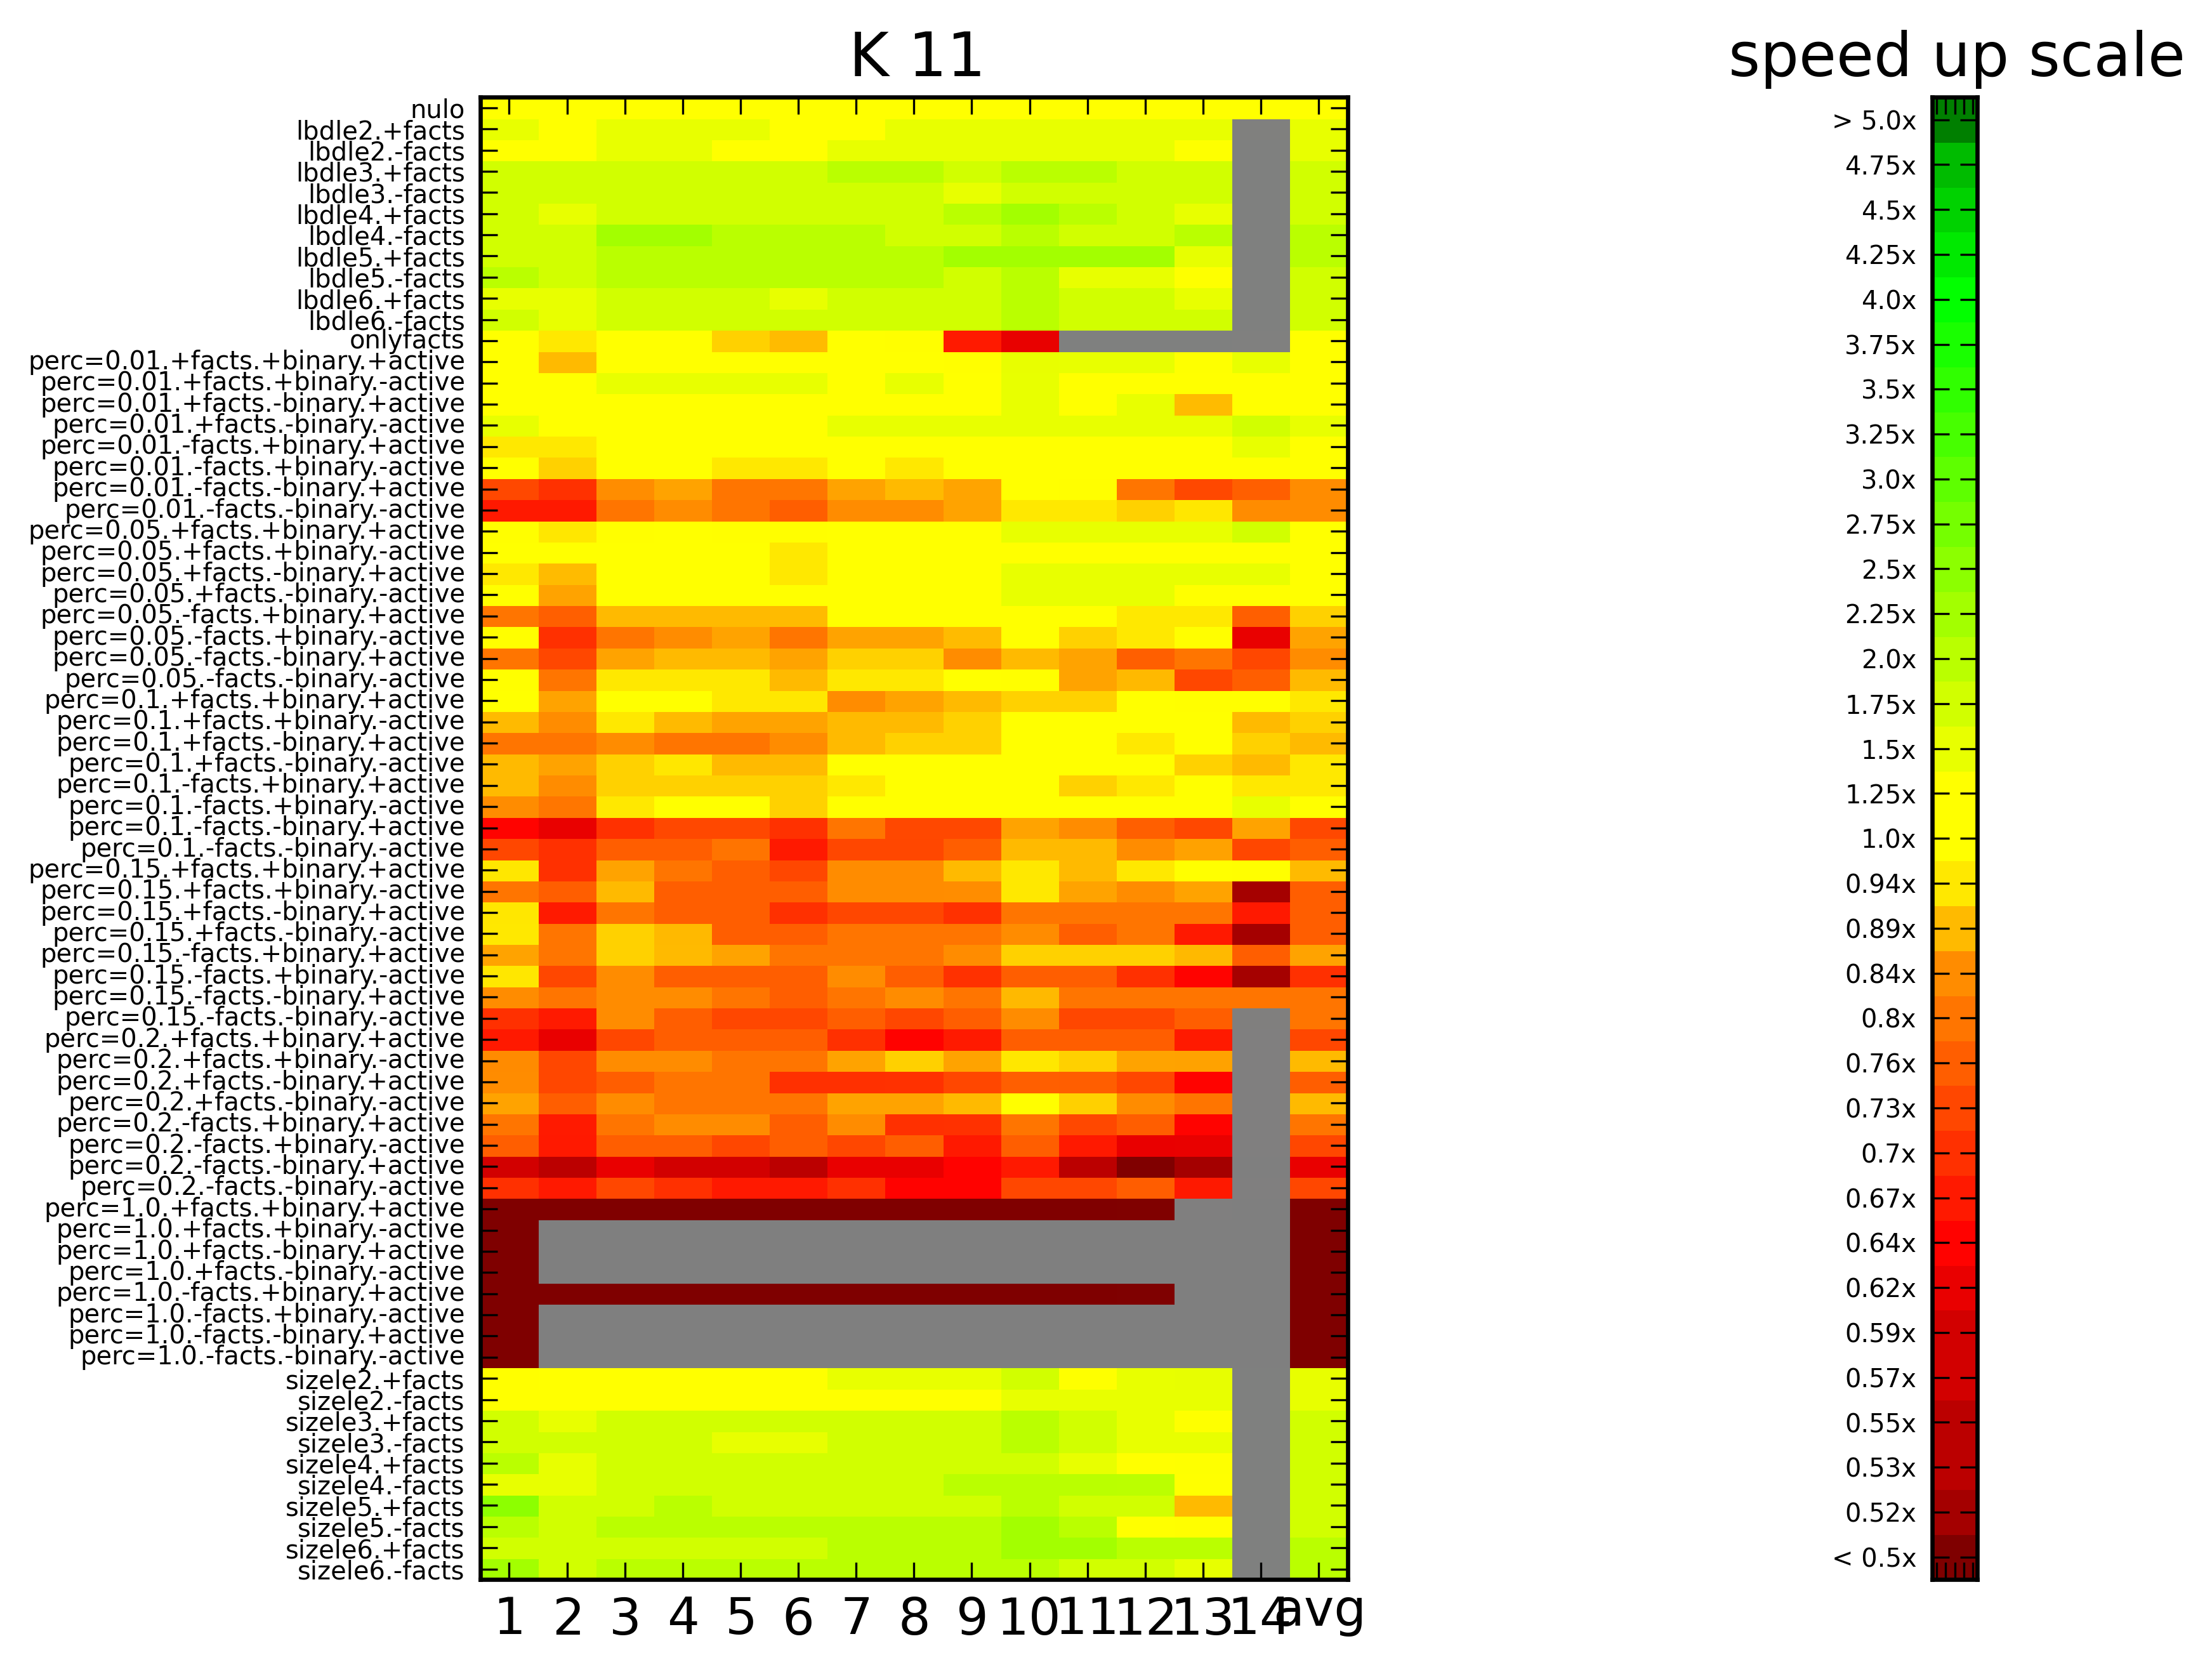
\includegraphics[scale=0.5]{resultados/k11_heat}
% 	%\caption{\emph{Workers}}
% \end{figure}
% \begin{figure}
% 	\centering
% 	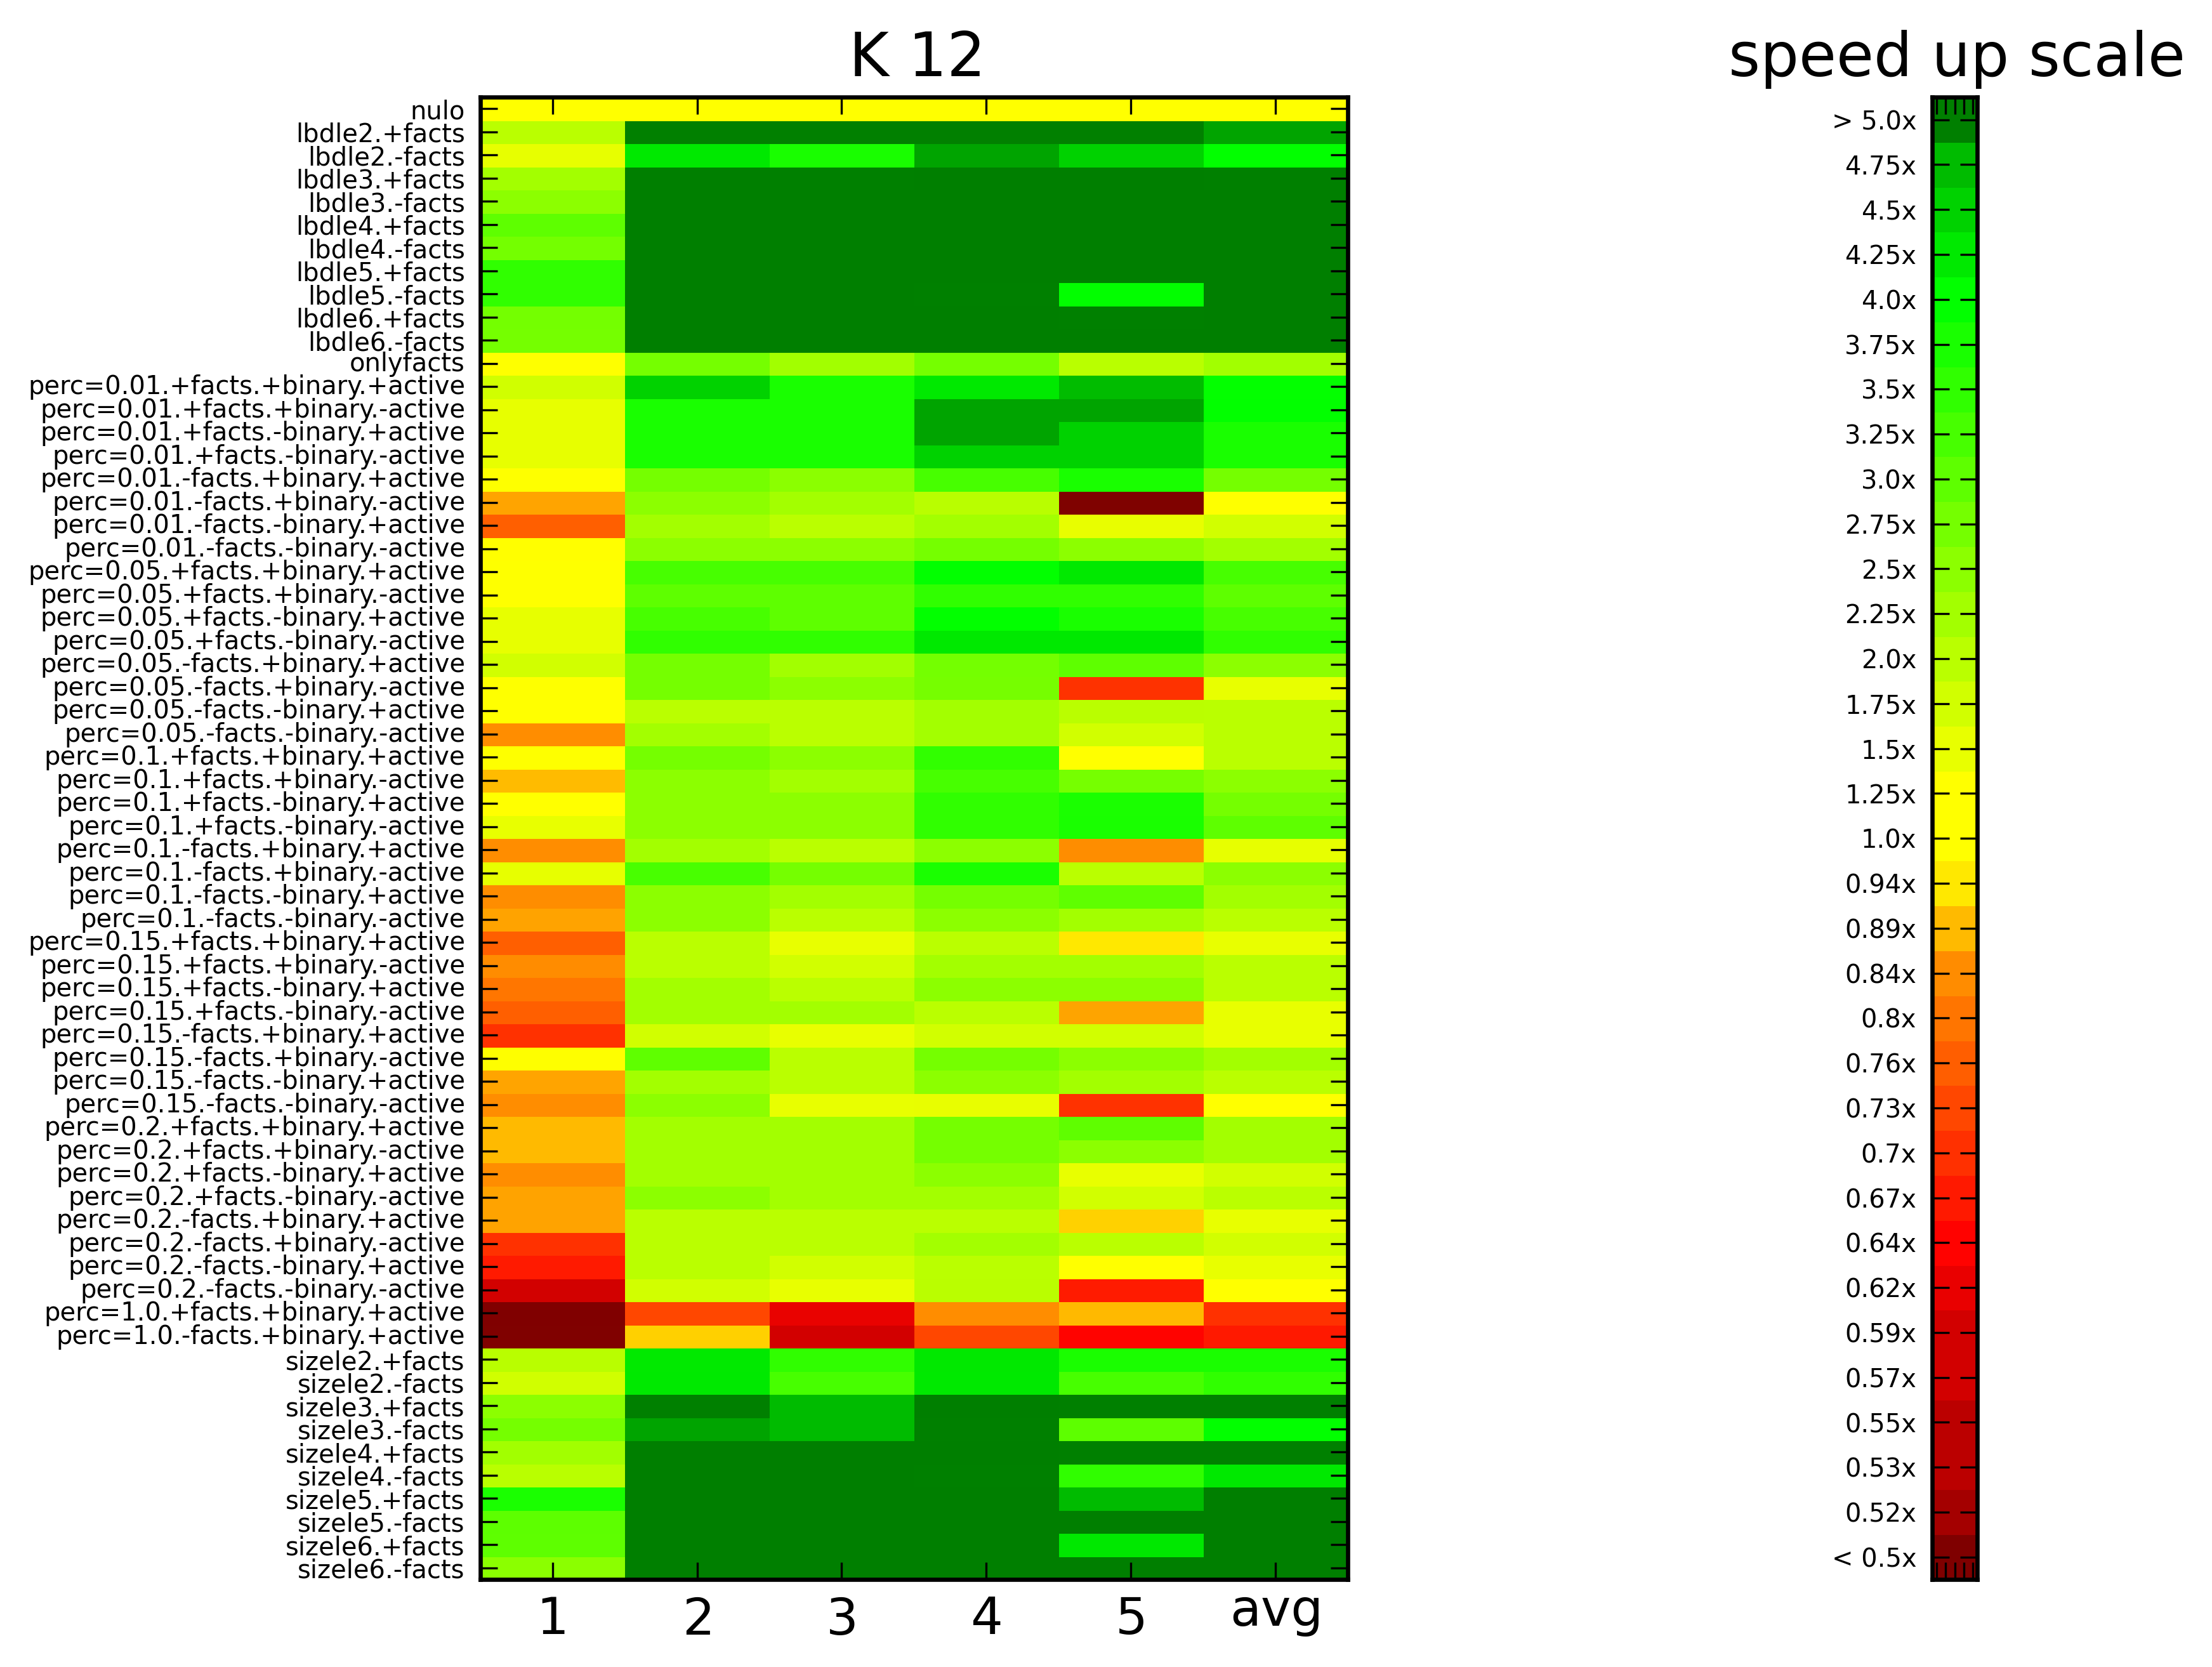
\includegraphics[scale=0.6]{resultados/k12_heat}
% 	%\caption{\emph{Workers}}
% \end{figure}
% \begin{figure}
% 	\centering
% 	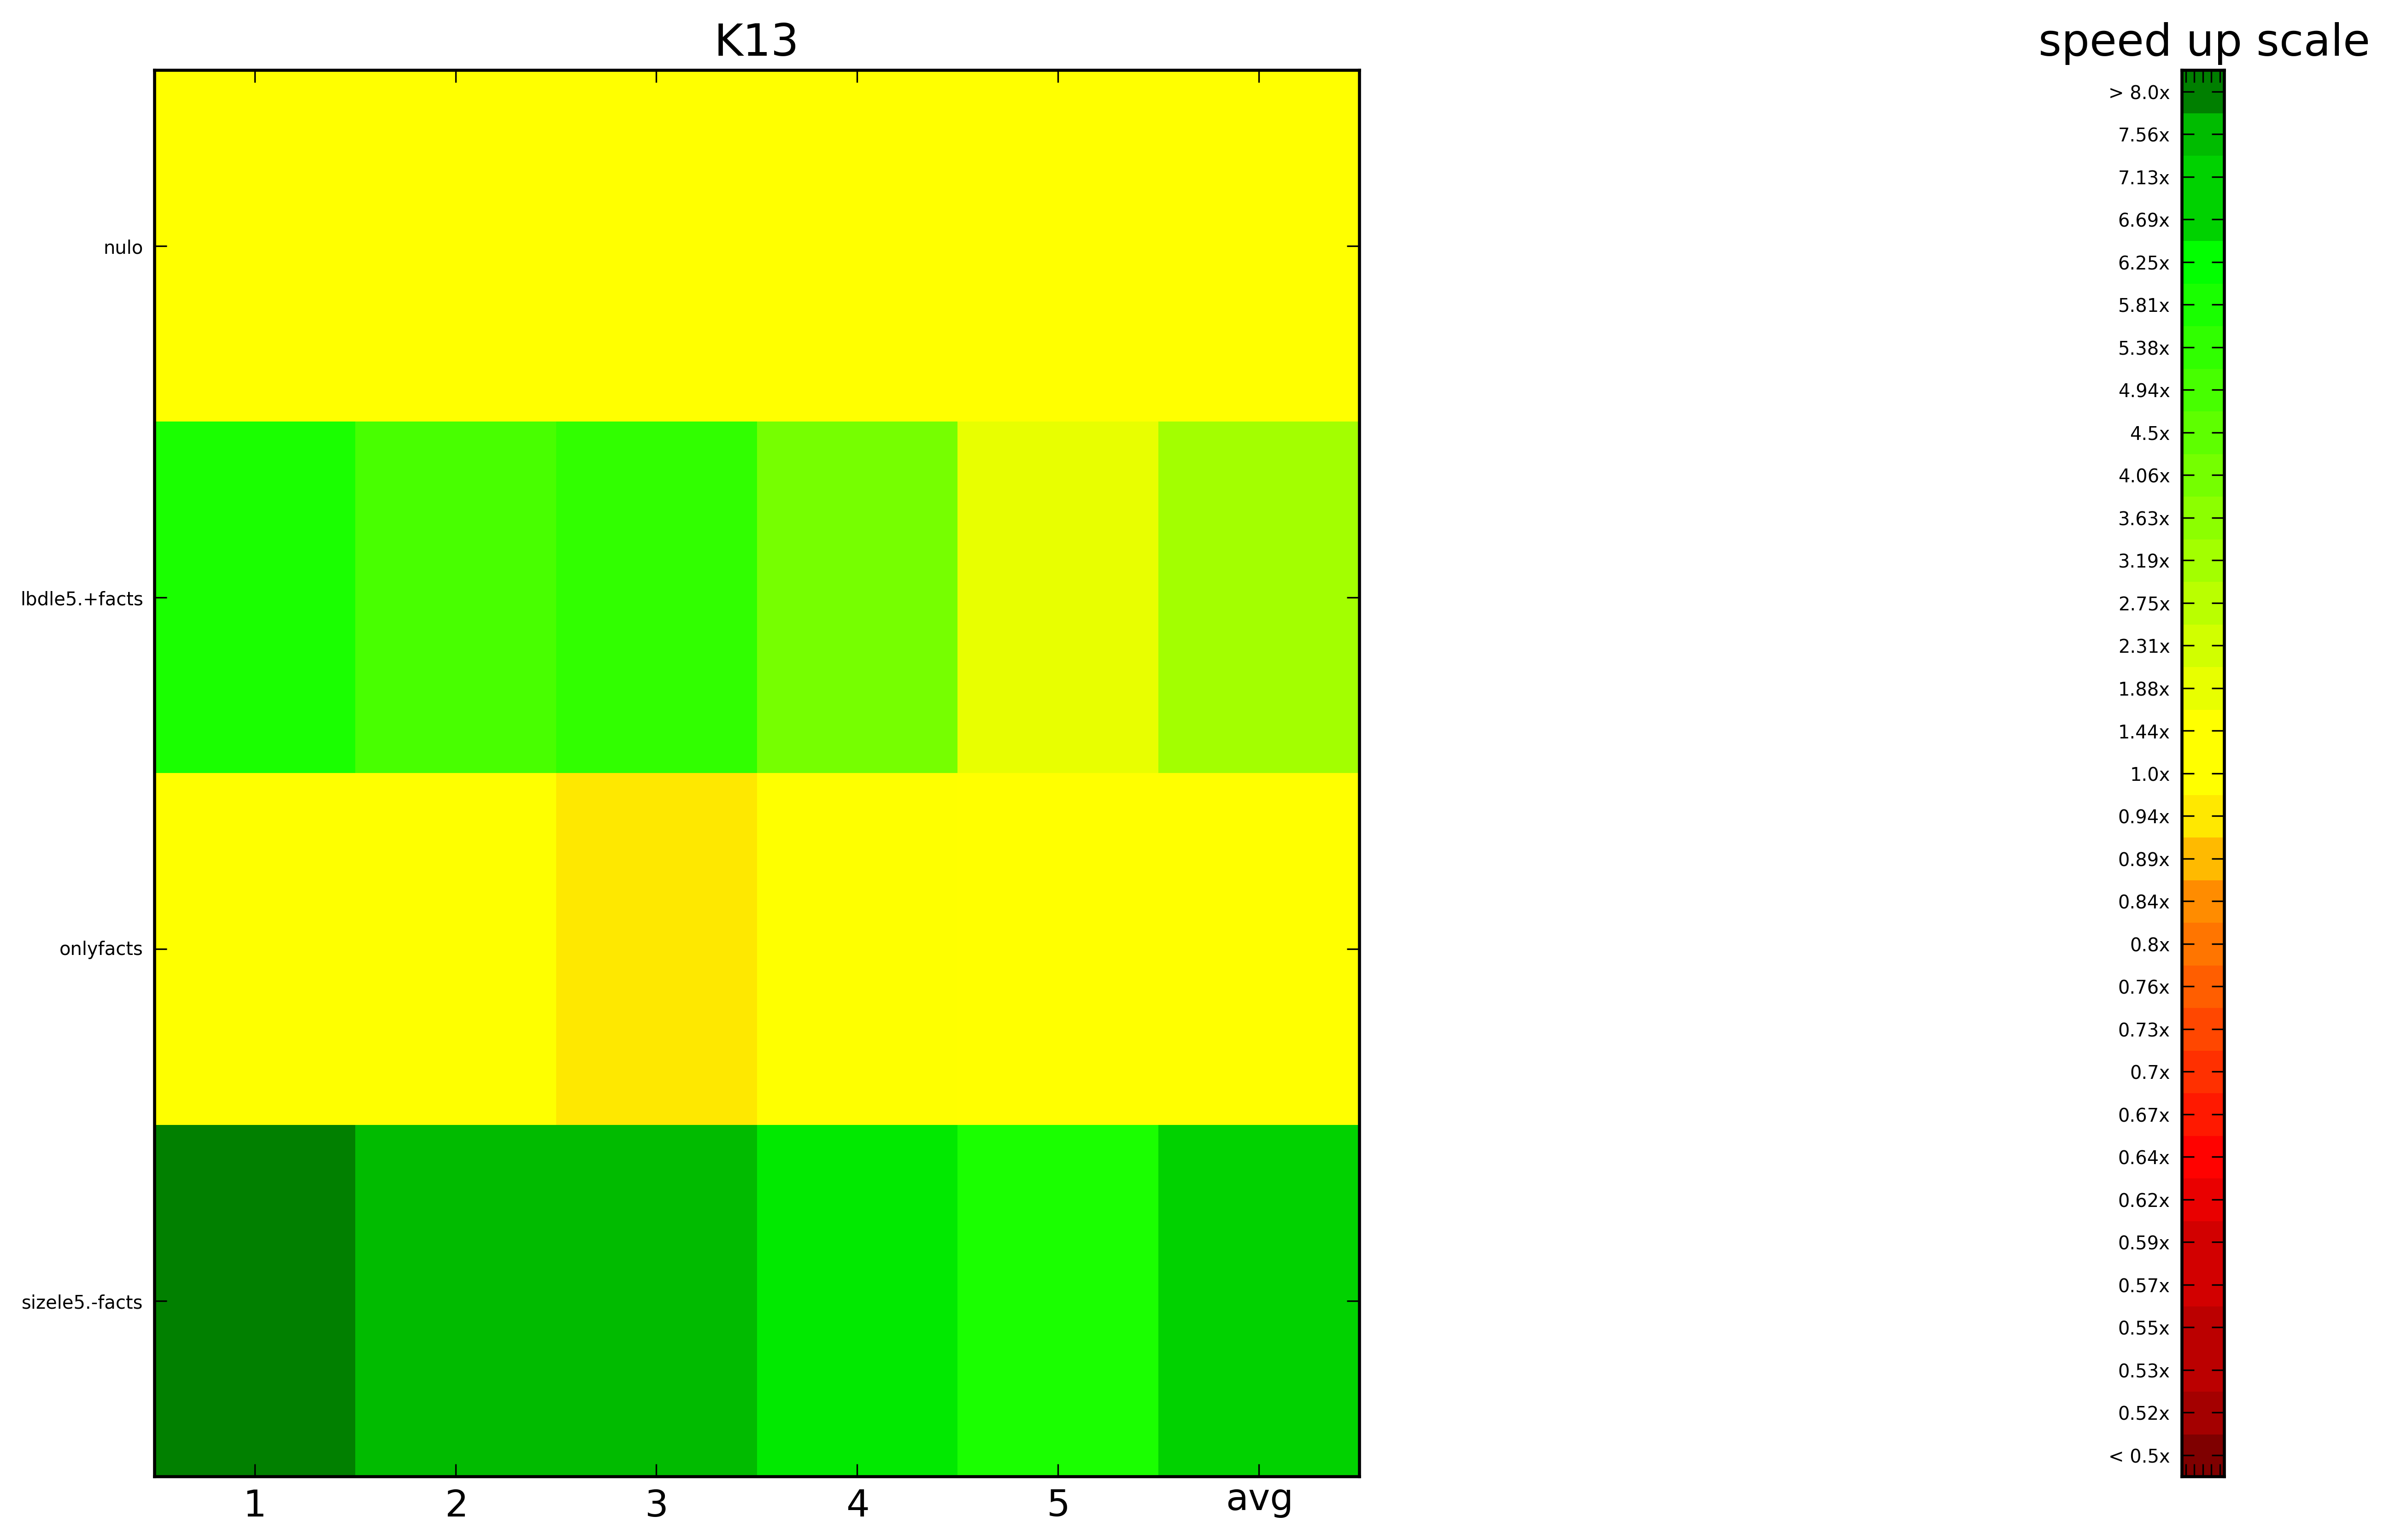
\includegraphics[scale=0.6]{resultados/k13_heat}
% 	%\caption{\emph{Workers}}
% \end{figure}

\hspace{-5em}
\begin{minipage}{\textwidth}
	\small
	\begin{tabular}{lrrr}
		\toprule
		criteria	&	worst speedup (x)	&	best speedup (x)	&	avg speedup (x) \\
		\cmidrule(r){1-4}
		lbdle2.+facts	&	0.68	&	4.91	&	1.97 \\
		lbdle2.-facts	&	0.71	&	3.84	&	1.24 \\
		lbdle3.+facts	&	0.78	&	5.16	&	1.41 \\
		lbdle3.-facts	&	0.75	&	5.71	&	1.69 \\
		lbdle4.+facts	&	0.64	&	6.80	&	1.68 \\
		lbdle4.-facts	&	0.79	&	5.83	&	1.83 \\
		lbdle5.+facts	&	0.69	&	6.74	&	1.64 \\
		lbdle5.-facts	&	0.77	&	5.25	&	2.14 \\
		lbdle6.+facts	&	0.76	&	5.79	&	1.95 \\
		lbdle6.-facts	&	0.70	&	6.08	&	1.94 \\
		\cmidrule(r){1-4}
		onlyfacts	&	\cellcolor{green}0.84	&	3.23	&	1.45 \\
		\cmidrule(r){1-4}
		perc=0.01.+facts.+binary.+active	&	\cellcolor{red}0.55	&	3.83	&	2.12 \\
		perc=0.01.+facts.+binary.-active	&	0.77	&	3.78	&	1.92 \\
		perc=0.01.+facts.-binary.+active	&	0.64	&	3.64	&	\cellcolor{red}1.19 \\
		perc=0.01.+facts.-binary.-active	&	0.65	&	3.50	&	1.39 \\
		perc=0.01.-facts.+binary.+active	&	0.74	&	2.73	&	1.91 \\
		perc=0.01.-facts.+binary.-active	&	0.69	&	2.38	&	1.30 \\
		perc=0.01.-facts.-binary.+active	&	0.74	&	\cellcolor{red}1.68	&	1.22 \\
		perc=0.01.-facts.-binary.-active	&	0.71	&	2.22	&	1.22 \\
		\cmidrule(r){1-4}
		sizele2.+facts	&	0.75	&	3.50	&	1.57 \\
		sizele2.-facts	&	0.81	&	3.32	&	\cellcolor{red}1.19 \\
		sizele3.+facts	&	\cellcolor{red}0.55	&	5.40	&	1.63 \\
		sizele3.-facts	&	0.75	&	3.87	&	1.39 \\
		sizele4.+facts	&	0.74	&	6.24	&	1.91 \\
		sizele4.-facts	&	0.72	&	4.21	&	1.81 \\
		sizele5.+facts	&	0.64	&	6.14	&	1.92 \\
		sizele5.-facts	&	0.58	&	\cellcolor{green}7.18	&	1.90 \\
		sizele6.+facts	&	0.72	&	5.08	&	2.17 \\
		sizele6.-facts	&	0.79	&	5.69	&	\cellcolor{green}2.61 \\
		\bottomrule
	\end{tabular}
	%\caption{Tiempo de ejecución (en segundos) distribuido vs. secuencial}
\end{minipage}